\chapter[Chapter 3: Research Methodology]{Research Methodology}

\section{Background}

\begin{figure}[hb]
	\centering
	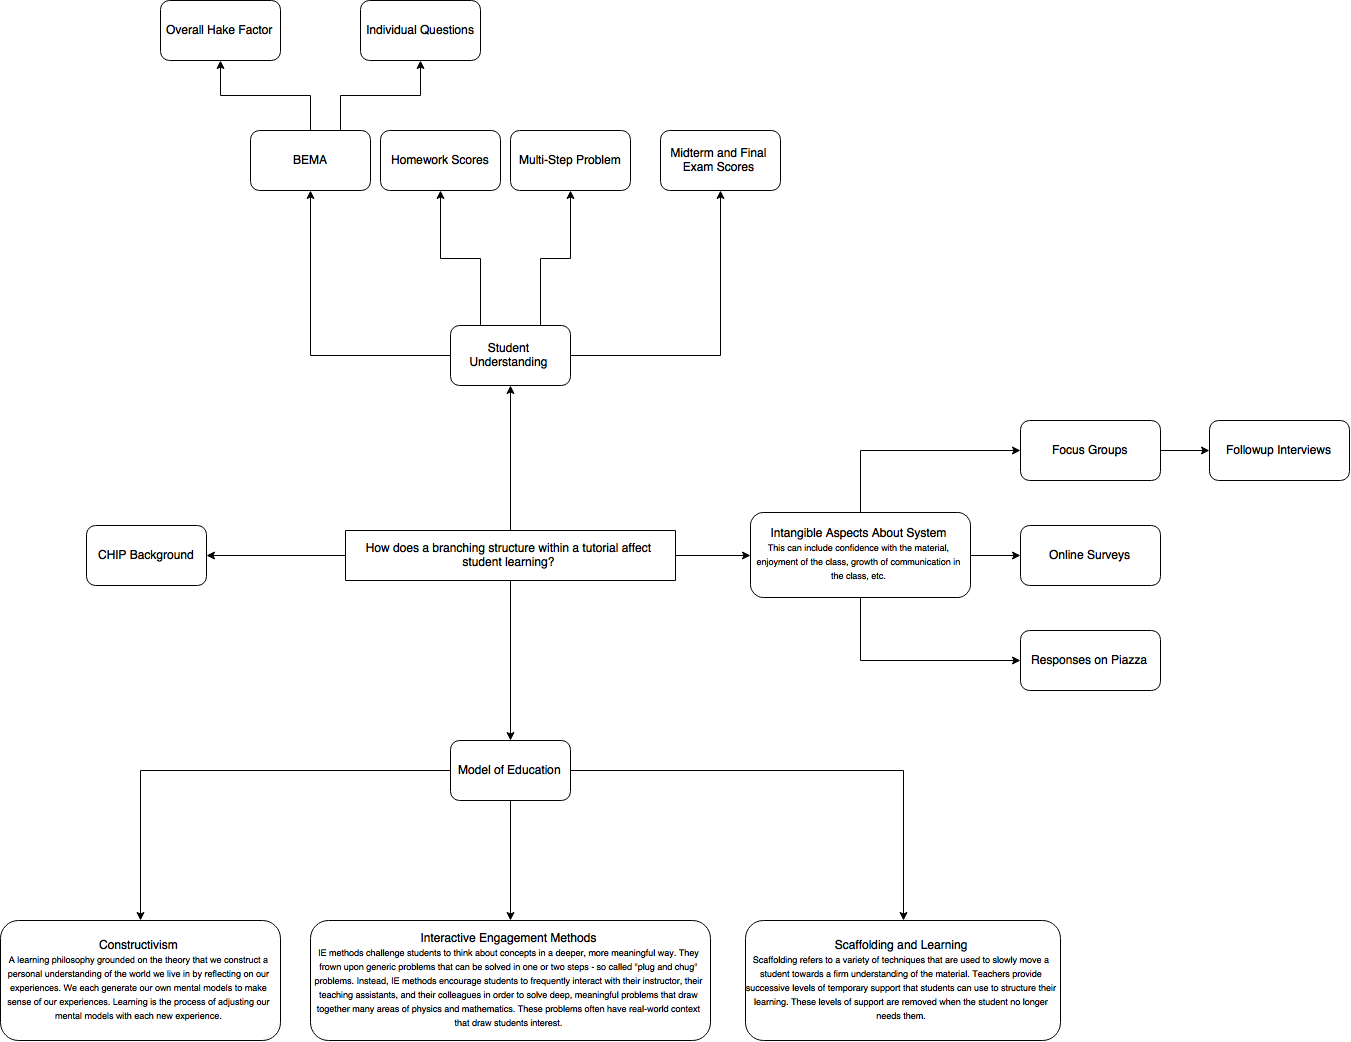
\includegraphics[width=6in]{img/chapter3/flowchart}
	\caption[Flowchart]{Flowchart}
\end{figure}

\subsection{Number of Students Impacted Each Year}

The combined yearly enrollment of PHYS
241 and PHYS 241D has a yearly average
enrollment of 1496 students from science and
engineering. Yearly enrollment in the online
portion of the course (started in Summer 2012)
has been increasing (Figure 2).

\section{Reflexivity}

Our team for the development and implementation of CITA on CHIP consists of Mr. Cyrus
Vandrevala (who will perform content development and coding to implement CITA on CHIP)
with oversight by Prof. Hisao Nakanishi and Prof. Laura Pyrak-Nolte. Mr. Vandrevala has been
a teaching assistant for PHYS 241 and PHYS 241D since Fall 2011, has coordinated the course
during summer sessions, and was instrumental in the development of the online course videos,
online recitation format, and online forum. Prof. Hisao Nakanishi has taught PHYS 241 and
more importantly is the “father” of CHIP. Professor Nakanishi takes an active role in ongoing
updates and improvements to content, functionality and robustness of the system. He also
addresses student questions sent through CHIP. Professor Laura Pyrak-Nolte has taught PHYS
241 since 2005, coordinated the course since Fall 2011 and is the online lecturer (i.e. in the
online videos) for PHYS 241D.

\section{Exams and Quizzes}



\section{Homework}

The ultimate test of CITA on CHIP is the ability to solve problems on exams. Student
performance on exam problems that are similar to CITA enhanced problems will be used to
determine if CITA improved learning outcomes, i.e. whether or not students have learned
specific problem solving strategies. We can correlate exam scores with:
• Which students use CITA (“A” students or students at all grade levels)
• When students started using CITA (before or after first exam, first homework, etc.)
• How many attempts on a problem are made before using CITA
• How many attempts to solve a problem are needed after using CITA
• After using CITA on one problem is it used on every problem
• Comparison of performance on CITA enhanced practice exams, non-CITA enhanced
practice exam and the performance on class exams.
In addition, we will use the standard assessment tool BEMA (Brief Electricity and Magnetism
Assessment) developed by Ding et al. (2006) to compare with our metrics. With an average total
yearly enrollment of 1500, sufficient statistics will be generated to determine the impact of CITA
on student learning

\section{Concept Assessment Instruments}

Concept inventories and assessment instruments are a useful method of assessing student knowledge of the material; however, they are not simply tests that can be quickly put together and administered year after year. Lindell and Ding describe how it takes years to determine the validity and reliability of the results of a given concept inventory. They describe how reliability (precision) and validity (accuracy) play a role in the inventories and cite how factors such as age, course structure, geography, language, delivery of the tests, and wording of questions can influence the results of the assessment\cite{lindell2012}.

\subsection{Brief Electricity and Magnetism Assessment (BEMA)}

The \gls{bema} was developed by Ruth Chabay, Bruce Sherwood, and Fred Reif in 1997. Although it was originally designed to measure student retention of electricity and magnetism concepts three months to five semesters after completing an introductory electricity and magnetism course, it is now often used to analyze student learning between the beginning and end of the semester. It is a useful tool to assess the understanding of electricity and magnetism concepts that are covered in a college-level calculus-based introductory physics course\cite{ding2006}.

The \gls{bema} is a multiple choice test consisting of qualitative questions and a few simple calculations. Lin Ding et al. performed an analysis of the \gls{bema}, showing that it is a reliable assessment tool for introductory electricity and magnetism courses\cite{ding2006}. We use the \gls{bema} extensively in our research to analyze student's understanding of the course material.

\subsection{Force Concept Inventory}

The \gls{fci}􏰁 is a multiple choice test that is used to measure a student's understanding of introductory mechanics. It is given at the beginning of an introductory mechanics course as a pre-test and again at the end of the course as a post-test. The pool of answers on the test are designed to correspond to common student misconceptions of mechanics; they were developed through a series of student interviews\cite{hestenes1992}.

Coletta et al. have observed a strong correlation between the normalized gain on the \gls{fci} and SAT scores. They go so far as to state that SAT scores might be a good indicator of the expected normalized gains within a classroom\cite{coletta2007}.

\section{Other Methods}

\section{Numerical Measures}

\subsection{Hake Factor (Gain Index)}

Normalized gain (G) vs. normalized gain <g>

\subsection{Gender Gap}

What am I trying to improve? What should I test?
Test scores -> Assess using PHYS 241 exam grades
Homework scores -> Assess using PHYS 241 homework grades
Quiz grades -> Assess using PHYS 241 quiz grades
Overall grades -> Assess using PHYS 241 course grades
Knowledge of qualitative electromagnetism concepts -> Assess using BEMA
Problem solving strategy -> Assess using worked out problems with custom rubrics
Student enjoyment in physics -> Personal interviews and class surveys
Student confidence in problem solving -> Personal interviews, worked out problems, and class surveys
Ability to make predictions in new and novel situations -> Give students advanced problems that they need to categorize
Ability to create diagrams -> Custom problems, draw a diagram from written directions
Ability to teach a concept -> Have them reteach the concept using a custom rubric
Close the gap between genders -> Test each gender and see if the gap closes
Close the gap between socioeconomic groups -> Test each group and see if the gap closes
Catch US students up to foreign students -> Test each group and see if the gap closes
Perform better in the lab (physical experiments) -> Create a lab assessment, maybe between 172 and 241
“Thinking like a physicist” -> Videotape how students solve interesting problems
The BEMA might not be a good way to assess CITA
Consider worked out problems
Track how far students get into problem using a custom rubric
Perhaps this can be implemented during recitation
Bruce and Ruth have a great presentation on their site as a demonstration

\section{Budget}

We are requesting support for graduate student, Mr. Vandrevala, for two years to perform the
work to achieve of objective of creating CITA on CHIP. In addition, funds for supplies for
research materials, electronic equipment and software are also requested. Funding is also
requested for travel for Mr. Vandrevala to attend education conferences to present our work.
The budget is given in Table 1 for a project period of two years (1/1/2015 – 12/31/2016).

\section{Development and Analysis Timeline}

The timeline for the development, implementation and assessment of CITA on CHIP is shown in Figure 1. In Spring 2015, the \gls{gui} will be updated for instructors and students, the
assessment tools will be tuned to included monitoring the impact of CITA, and CITA enabled
problems will be added in preparation for the summer courses. CITA enabled homework
problems will be rolled-out in Summer 2015 and provide important feedback from students and
instructors on the ease of use, helpfulness of suggestions, and acquisition of
appropriate/necessary learning data needed for assessment. Concurrently, CITA will be
expanded to practice exam problems during Summer 2015 along with any improvements based
on initial user feedback. Summer enrollment in 2014 was on the order of 150 students. The next
challenge is to test the system in Fall 2015 with projected enrollment between 775 – 800
students. The Fall 2015 student learning data will provide sufficient statistics to begin the
assessment and efficacy of CITA on CHIP. In addition, work will continue on expanding CITA
with more homework problems and exams from Spring 2015 and Summer 2015. Our approach
is to continually upgrade CITA based on student and instructor feedback. At the end of Fall
2016, we will meet and assess the impact of
CITA on student learning.

\begin{table}[!ht]
  \centering
  \begin{tabular}{|l|l|l|l|}
    \hline
    \textbf{Date} & \textbf{Events} & \textbf{Notes}\\
	\hline
	Spring 2015 & Create Branching Help Button in \gls{chip} & Spearheaded by Dr. Hisao Nakanishi\\
	& Create \gls{cita} Homework Problems & hi\\
	\hline
	Summer 2015 & Create \gls{cita} Homework Problems & Finish\\
	& Beta Test of \gls{cita} Homework Problems & hi\\
	\hline
	Fall 2015 & Update \gls{gui} for \gls{chip} & Pending\\
	& Update \gls{gui} for \gls{cita} & Pending\\
	& Update Assessment Tools on \gls{chip} & Pending\\
	\hline
	Spring 2016 & Expand \gls{cita} Problems & Pending\\
	& Analyze \gls{cita} Data from Fall 2015 & Pending\\
	Summer 2016 & 2 & 3\\
	Fall 2016 & 2 & 3\\
	& Expand \gls{cita} Problems & Pending\\
	\hline
  \end{tabular}
  \caption{Project Timeline}
  \label{tab:timeline}
\end{table}